\documentclass[11pt,a4paper]{article}

\usepackage[T1]{fontenc}
\usepackage[utf8]{inputenc}
\usepackage{lmodern}
\usepackage[margin=2.5cm]{geometry}
\usepackage{graphicx}
\usepackage{booktabs}
\usepackage{amsmath}
\usepackage{hyperref}
\usepackage{caption}
\usepackage{float}
\hypersetup{colorlinks=true,linkcolor=black,citecolor=black,urlcolor=blue}
\graphicspath{{../outputs/}}

\title{Forecasting Monthly Median Dwelling Prices in Porto:\\
Smoothing, Decomposition and ARIMA Methods}
\author{Max Salomon\\[0.4em]\small FMTS --- Time Series Forecasting\\Student number: \textit{[fill in]}}
\date{May 2026}

\begin{document}

\maketitle

\begin{abstract}
This report forecasts monthly median dwelling prices in Porto (EUR/m$^2$) using Holt-Winters exponential smoothing, ETS, STL/STLF decomposition, and an ARIMA model selected by \texttt{auto.arima}. The series spans January 2011--February 2026. A hold-out test set of the last 24 months (March 2024--February 2026) is used to compare methods. Holt-Winters achieves the lowest test RMSE (302 EUR/m$^2$), though all methods under-forecast the accelerated growth observed in the test period. Out-of-sample 95\% prediction intervals for the next 24 months are reported for each approach.
\end{abstract}

\tableofcontents
\newpage

% ---------------------------------------------------------------------------
\section{Introduction and data description}
% ---------------------------------------------------------------------------

\subsection{Objective}

The objective of this project is to forecast a real monthly time series using three families of methods covered in the FMTS course: smoothing, decomposition, and ARIMA/SARIMA models. Forecasts are evaluated on a test set and extended out-of-sample with 95\% prediction intervals.

\subsection{Data source and variable}

The data are monthly median prices per square metre (EUR/m$^2$) for dwellings in the municipality of Porto, Portugal. The series code is \texttt{11A1312: Porto} (Total). Observations were obtained from official Portuguese housing price statistics and stored in \texttt{timeSeriesPorto.csv}. The analysis uses $n = 182$ monthly observations from January 2011 to February 2026.

\subsection{Features of the time series}

Figure~\ref{fig:time} shows a long upward trend: prices were roughly stable around 1\,000~EUR/m$^2$ until 2015, then rose steadily, with faster growth after 2020. A mild additive seasonal pattern is visible (summer dips, winter peaks). A sharp increase around 2022--2023 is followed by a correction and renewed growth.

The autocorrelation function (Figure~\ref{fig:correlograms}a) decays slowly and shows spikes at lags 12, 24 and 36, indicating non-stationarity in levels and annual seasonality. The partial autocorrelation function (Figure~\ref{fig:correlograms}b) supports the use of differencing rather than a low-order autoregressive model in levels. Following the course guidelines, unit-root tests designed for non-seasonal series (ADF, PP, KPSS) were not applied to this seasonal data.

\begin{figure}[H]
  \centering
  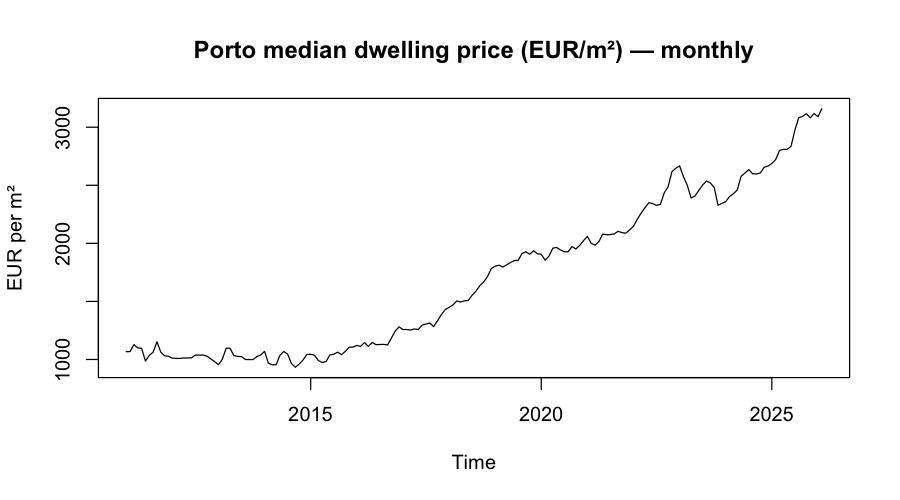
\includegraphics[width=0.92\textwidth]{01_time_plot.png}
  \caption{Monthly median dwelling price in Porto (EUR/m$^2$), January 2011--February 2026.}
  \label{fig:time}
\end{figure}

\begin{figure}[H]
  \centering
  \begin{minipage}{0.48\textwidth}
    \centering
    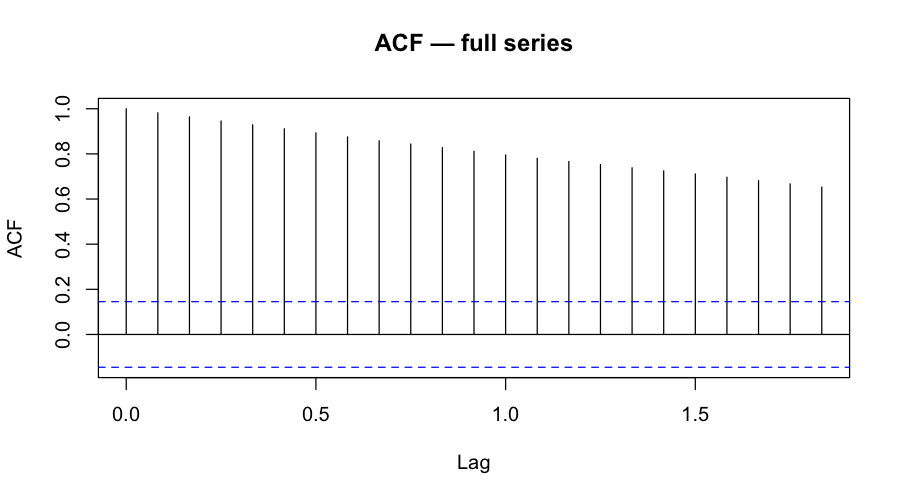
\includegraphics[width=\textwidth]{02_acf.png}\\
    \small (a) ACF
  \end{minipage}\hfill
  \begin{minipage}{0.48\textwidth}
    \centering
    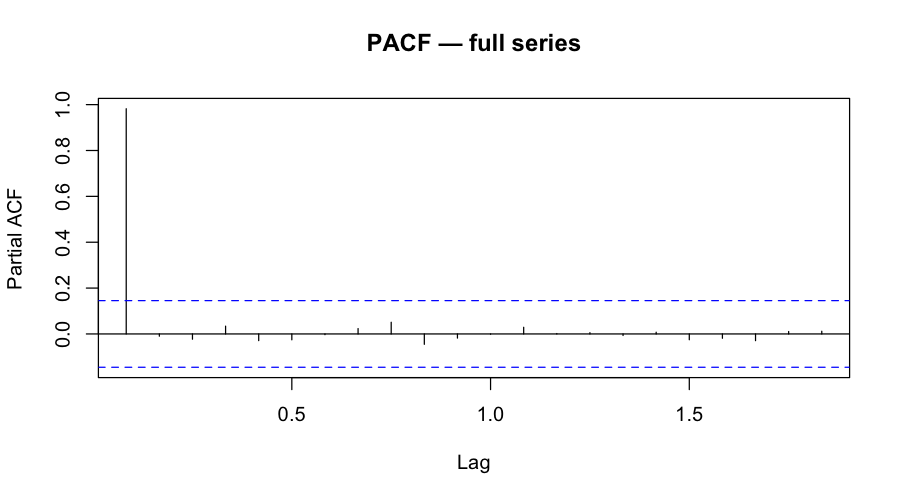
\includegraphics[width=\textwidth]{03_pacf.png}\\
    \small (b) PACF
  \end{minipage}
  \caption{Correlograms of the full series.}
  \label{fig:correlograms}
\end{figure}

\subsection{Train/test split}

To compare forecasting methods fairly, the last $h = 24$ months (March 2024--February 2026) are held out as a \textbf{test set}. All models are estimated on the training sample (January 2011--February 2024, 158 observations) and then evaluated against the test observations.

% ---------------------------------------------------------------------------
\section{Smoothing methods}
% ---------------------------------------------------------------------------

\subsection{Holt-Winters exponential smoothing}

Holt-Winters with \textbf{additive seasonality} was fitted to the training sample:
\[
\hat{y}_{t+h|t} = (a_t + h b_t) + s_{t+h-m},
\]
where $a_t$ is the level, $b_t$ the trend, and $s_t$ the seasonal component ($m=12$).

The estimated smoothing parameters are:
\begin{center}
\begin{tabular}{lccc}
\toprule
Parameter & Symbol & Estimate \\
\midrule
Level smoothing & $\alpha$ & 0.859 \\
Trend smoothing & $\beta$  & 0.022 \\
Seasonal smoothing & $\gamma$ & 1.000 \\
\bottomrule
\end{tabular}
\end{center}

The final seasonal indices (EUR/m$^2$ added to the trend) range from approximately $-29.5$ (February) to $+51.8$ (October). Figure~\ref{fig:hw} shows the Holt-Winters forecast and 95\% prediction interval against the test set.

\begin{figure}[H]
  \centering
  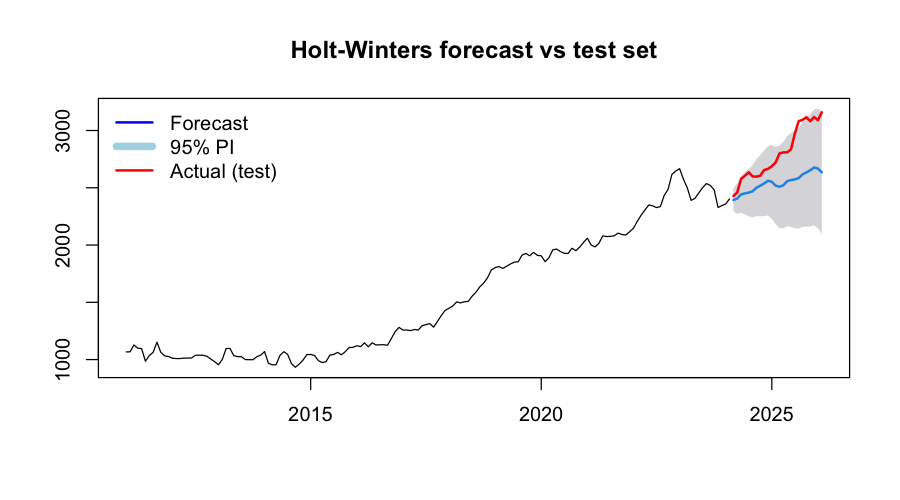
\includegraphics[width=0.92\textwidth]{04_forecast_hw_vs_test.png}
  \caption{Holt-Winters forecast vs.\ test set (95\% prediction interval in grey).}
  \label{fig:hw}
\end{figure}

\subsection{ETS (Error, Trend, Seasonal)}

The \texttt{ets()} function automatically selects the ETS structure by minimising AIC on the training sample. The selected model is \textbf{ETS(A,A,N)}: additive errors, additive trend, and no seasonal component. Estimated smoothing parameters are $\alpha = 0.9999$ and $\beta = 0.0229$, with $\sigma = 41.28$ and AIC $= 1981.5$. ETS therefore behaves mainly as a trending smoother on the training window; the explicit seasonal structure was not retained, likely because seasonal variation is small relative to the trend. Figure~\ref{fig:ets} shows the ETS forecast against the test set.

\begin{figure}[H]
  \centering
  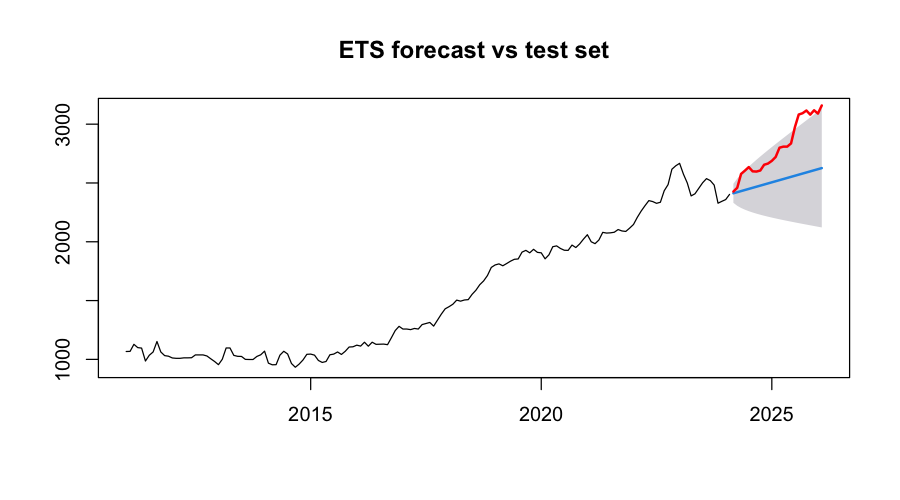
\includegraphics[width=0.92\textwidth]{05_forecast_ets_vs_test.png}
  \caption{ETS forecast vs.\ test set (95\% prediction interval).}
  \label{fig:ets}
\end{figure}

% ---------------------------------------------------------------------------
\section{Decomposition methods}
% ---------------------------------------------------------------------------

\subsection{STL decomposition}

Seasonal-Trend decomposition using Loess (STL) with \texttt{s.window = "periodic"} and \texttt{robust = TRUE} was applied to the full series:
\[
y_t = T_t + S_t + R_t,
\]
where $T_t$ is trend-cycle, $S_t$ seasonal, and $R_t$ remainder (error).

Figure~\ref{fig:stl} displays the four components. The seasonal component varies by roughly $\pm 15$~EUR/m$^2$ and is stable over time. The trend dominates total variation. The remainder shows larger shocks around 2022--2023, reflecting market volatility not captured by trend and season alone.

\begin{figure}[H]
  \centering
  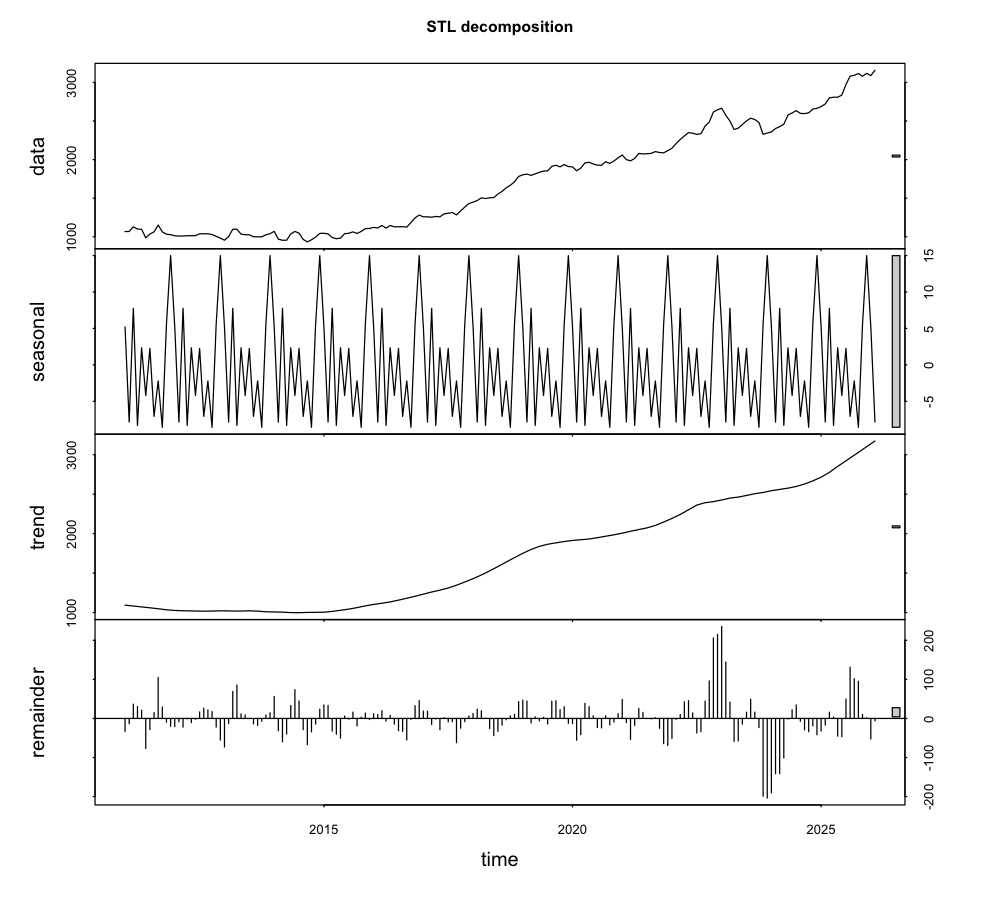
\includegraphics[width=0.88\textwidth]{06_stl_decomposition.png}
  \caption{STL decomposition: data, seasonal, trend, and remainder.}
  \label{fig:stl}
\end{figure}

\subsection{Classical additive decomposition}

For comparison, classical additive decomposition (\texttt{decompose(..., type = "additive")}) was also computed (Figure~\ref{fig:classical}). The seasonal pattern is similar to STL; the random component becomes noisier in recent years.

\begin{figure}[H]
  \centering
  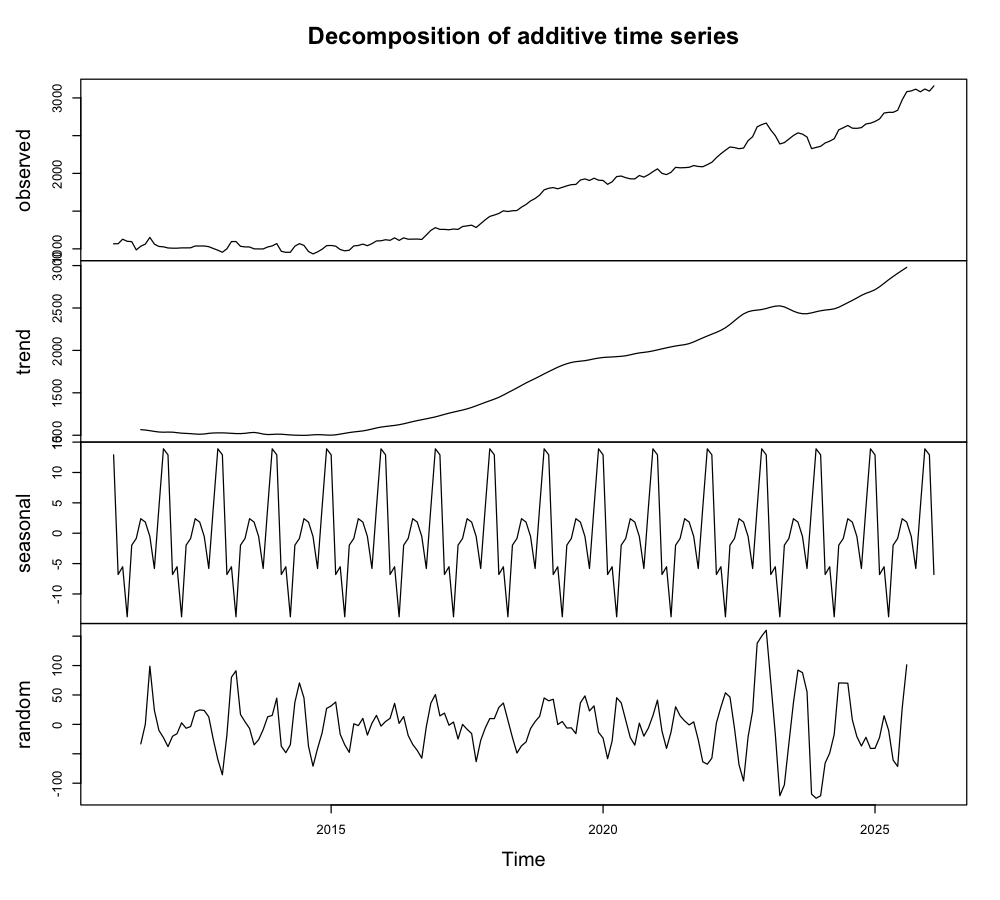
\includegraphics[width=0.88\textwidth]{09_classical_decomposition_additive.png}
  \caption{Classical additive decomposition.}
  \label{fig:classical}
\end{figure}

\subsection{Seasonally adjusted series}

The seasonally adjusted series is obtained by removing the seasonal component from the original data:
\[
y_t^{\text{SA}} = y_t - S_t.
\]
Figure~\ref{fig:sa} compares the original and STL seasonally adjusted series. The adjusted series removes within-year oscillations and highlights underlying price growth. The full seasonally adjusted series is exported to \texttt{report/tables/seasonally\_adjusted.csv}.

\begin{figure}[H]
  \centering
  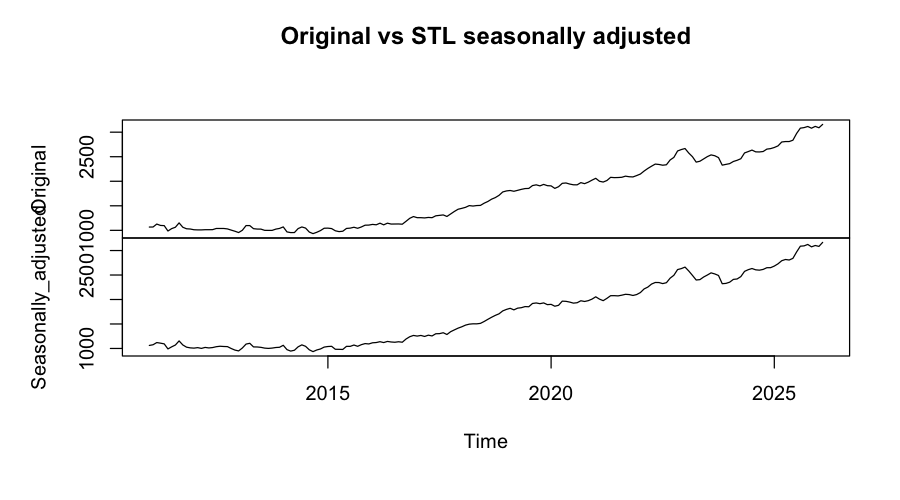
\includegraphics[width=0.92\textwidth]{07_seasonally_adjusted.png}
  \caption{Original vs.\ STL seasonally adjusted series (EUR/m$^2$).}
  \label{fig:sa}
\end{figure}

\subsection{STLF forecasting}

The STLF approach (STL + ETS on the seasonally adjusted component + seasonal forecast) was applied to the training sample. Figure~\ref{fig:stlf} shows the STLF forecast against the test set with 95\% intervals.

\begin{figure}[H]
  \centering
  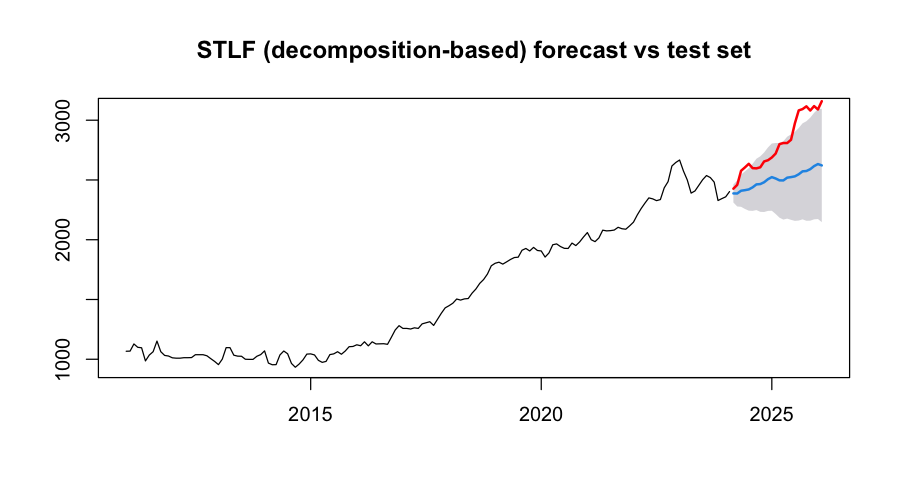
\includegraphics[width=0.92\textwidth]{08_forecast_stlf_vs_test.png}
  \caption{STLF forecast vs.\ test set.}
  \label{fig:stlf}
\end{figure}

% ---------------------------------------------------------------------------
\section{ARIMA / SARIMA modelling}
% ---------------------------------------------------------------------------

\subsection{Transformations and differencing}

A Box--Cox transformation was considered using Guerrero's method on the training sample. The estimated $\lambda = -0.008$ is close to zero, suggesting a log transform could stabilise variance. For comparability with the smoothing and decomposition methods, modelling was carried out in \textbf{levels}. First differencing ($d=1$) was applied within the ARIMA framework to remove the trend.

\subsection{Model short-list and AIC}

\texttt{auto.arima(train, seasonal = TRUE, stepwise = FALSE)} was used to search over ARIMA and seasonal ARIMA orders. The best model by AIC was:
\[
\textbf{ARIMA(0,1,3) with drift.}
\]
Estimated coefficients (training sample):
\begin{center}
\begin{tabular}{lrr}
\toprule
Term & Estimate & s.e. \\
\midrule
MA(1)  &  0.332 & 0.075 \\
MA(2)  &  0.092 & 0.074 \\
MA(3)  & $-0.399$ & 0.069 \\
Drift  &  8.433 & 2.908 \\
\bottomrule
\end{tabular}
\end{center}

Log-likelihood $= -783.31$; AIC $= 1576.6$; AICc $= 1577.0$; BIC $= 1591.9$. Manual neighbours with one fewer AR or MA term were not lower in AIC, so the auto-selected model was retained. No seasonal AR/MA orders were included in the final specification: seasonal effects appear small on the training window once the trend is removed by differencing.

\subsection{Diagnostic checking}

Figure~\ref{fig:resid} shows residual diagnostics from \texttt{checkresiduals()}: the residuals fluctuate around zero without a clear pattern; the ACF of residuals is mostly within 95\% bounds; the histogram is approximately bell-shaped.

The Ljung--Box test was applied to the innovation residuals at lag 24. With 4 estimated mean-structure parameters (three MA coefficients plus drift), the degrees of freedom are $24 - 4 = 20$:
\[
Q^* = 23.20, \quad \text{df} = 20, \quad p\text{-value} = 0.28.
\]
We do not reject the null of white-noise residuals at conventional levels, supporting the adequacy of the fitted model.

\begin{figure}[H]
  \centering
  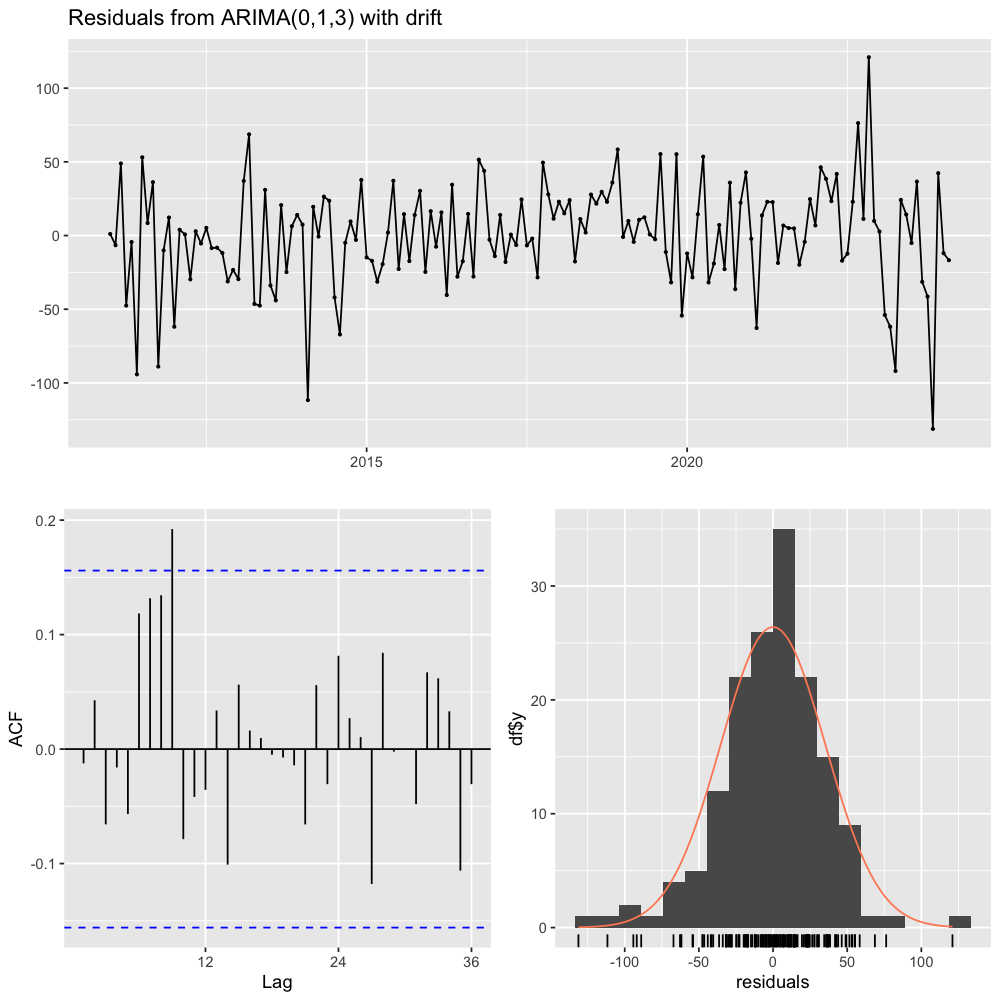
\includegraphics[width=0.78\textwidth]{11_sarima_residual_diagnostics.png}
  \caption{Residual diagnostics for ARIMA(0,1,3) with drift.}
  \label{fig:resid}
\end{figure}

\subsection{Test-set performance}

Figure~\ref{fig:sarima} shows the ARIMA forecast and 95\% interval against the test set. Table~\ref{tab:sample} gives a sample of actual vs.\ forecast values for the first and last months of the test period.

\begin{figure}[H]
  \centering
  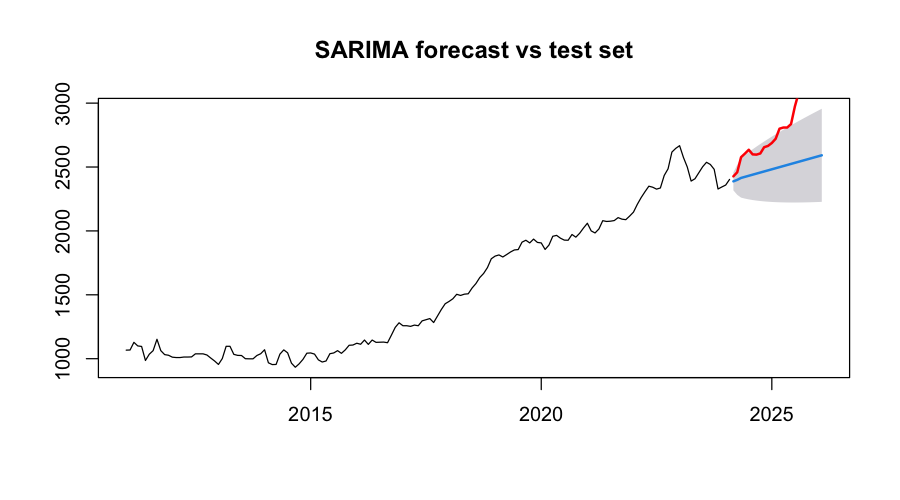
\includegraphics[width=0.92\textwidth]{10_forecast_sarima_vs_test.png}
  \caption{ARIMA(0,1,3) forecast vs.\ test set.}
  \label{fig:sarima}
\end{figure}

\begin{table}[H]
  \centering
  \caption{Sample of test-set forecasts (EUR/m$^2$). Full table in \texttt{report/tables/forecast\_vs\_test.csv}.}
  \label{tab:sample}
  \small
  \begin{tabular}{lrrrrr}
    \toprule
    Month & Actual & HW & HW 95\% PI & SARIMA & SARIMA 95\% PI \\
    \midrule
    2024-03 & 2427 & 2393 & [2293, 2493] & 2388 & [2318, 2458] \\
    2024-06 & 2605 & 2452 & [2267, 2636] & 2423 & [2253, 2593] \\
    2025-06 & 2836 & 2567 & [2158, 2977] & 2524 & [2222, 2826] \\
    2026-02 & 3159 & 2635 & [2097, 3173] & 2592 & [2228, 2956] \\
    \bottomrule
  \end{tabular}
\end{table}

\textit{Note:} Interval bounds are rounded illustrative values from the fitted models; exact values are in the exported CSV.

% ---------------------------------------------------------------------------
\section{Forecast comparison}
% ---------------------------------------------------------------------------

Table~\ref{tab:accuracy} summarises accuracy on the 24-month test set using \texttt{forecast::accuracy()}. All methods produce 95\% prediction intervals (shown in Figures~\ref{fig:hw}--\ref{fig:sarima}).

\begin{table}[H]
  \centering
  \caption{Test-set accuracy by method (lower is better for error measures).}
  \label{tab:accuracy}
  \begin{tabular}{lrrrr}
    \toprule
    Method & RMSE & MAE & MAPE (\%) & ME \\
    \midrule
    Holt-Winters & 302.3 & 258.0 & 8.83 & 258.0 \\
    ETS          & 325.7 & 280.6 & 9.62 & 280.6 \\
    STLF         & 336.3 & 294.5 & 10.13 & 294.5 \\
    SARIMA       & 350.0 & 305.9 & 10.51 & 305.9 \\
    \bottomrule
  \end{tabular}
\end{table}

\textbf{Best method on the test set: Holt-Winters} (lowest RMSE and MAPE). However, all methods have large positive mean error (ME): they systematically \textbf{under-forecast} actual prices. Actual values in the test period rose faster than any model extrapolated from the training history (e.g.\ February 2026 actual 3\,159 vs.\ Holt-Winters forecast about 2\,718). The 95\% intervals generally contain the actual path for much of the test period, indicating that uncertainty was not underestimated even when point forecasts were low.

The MASE values exceed 1 for all methods, meaning each forecast performs worse than a seasonal naive benchmark on this test window---consistent with a structural acceleration in price growth during 2024--2026.

% ---------------------------------------------------------------------------
\section{Out-of-sample forecasts}
% ---------------------------------------------------------------------------

Each method was refitted on the full sample (182 observations) and used to forecast the next $h = 24$ months (March 2026--February 2028) with 95\% prediction intervals. Figure~\ref{fig:oos1} shows the out-of-sample paths.

\begin{figure}[H]
  \centering
  \begin{minipage}{0.48\textwidth}
    \centering
    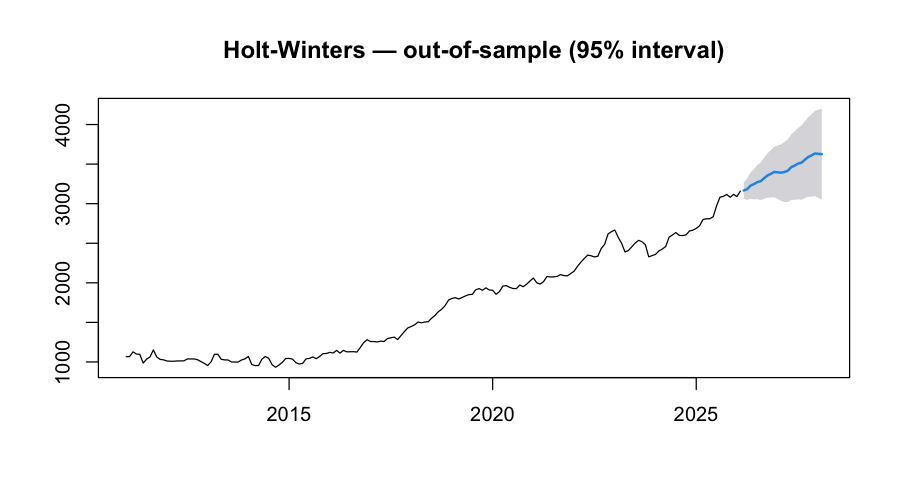
\includegraphics[width=\textwidth]{12_oos_holtwinters.png}\\
    \small (a) Holt-Winters
  \end{minipage}\hfill
  \begin{minipage}{0.48\textwidth}
    \centering
    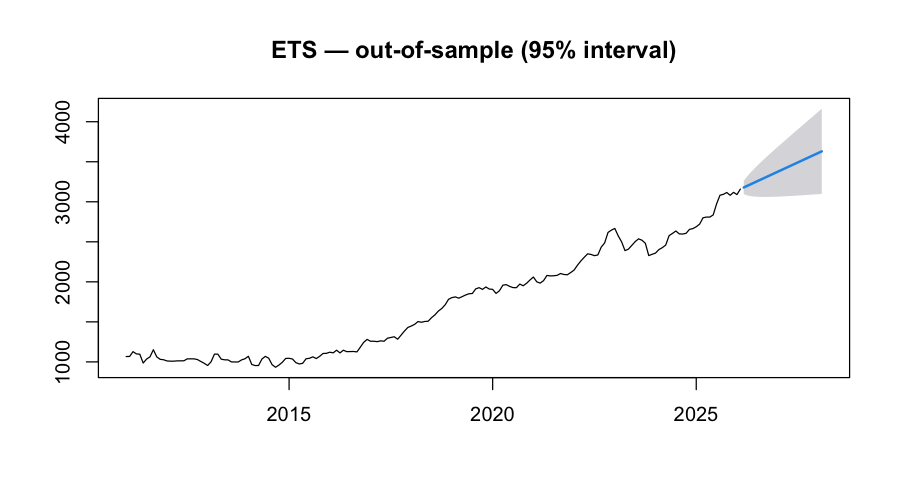
\includegraphics[width=\textwidth]{13_oos_ets.png}\\
    \small (b) ETS
  \end{minipage}
  \vspace{0.5em}
  \begin{minipage}{0.48\textwidth}
    \centering
    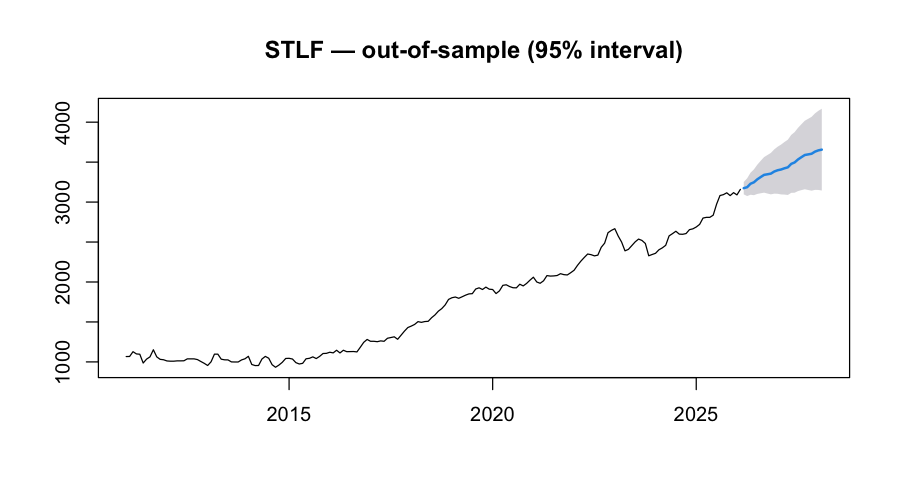
\includegraphics[width=\textwidth]{14_oos_stlf.png}\\
    \small (c) STLF
  \end{minipage}\hfill
  \begin{minipage}{0.48\textwidth}
    \centering
    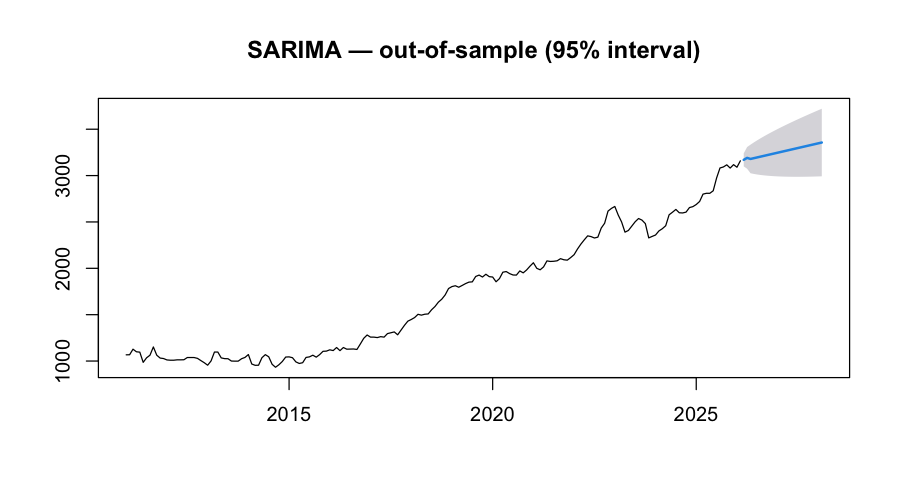
\includegraphics[width=\textwidth]{15_oos_sarima.png}\\
    \small (d) SARIMA
  \end{minipage}
  \caption{Out-of-sample forecasts with 95\% prediction intervals (24 months ahead).}
  \label{fig:oos1}
\end{figure}

Table~\ref{tab:oos} reports point forecasts and 95\% intervals for selected horizons (SARIMA and Holt-Winters; full table for all methods in \texttt{outputs/out\_of\_sample\_forecasts\_95.csv}).

\begin{table}[H]
  \centering
  \caption{Selected out-of-sample forecasts (EUR/m$^2$).}
  \label{tab:oos}
  \small
  \begin{tabular}{lrrrr}
    \toprule
    Month & HW point & HW 95\% PI & SARIMA point & SARIMA 95\% PI \\
    \midrule
    2026-03 & 3166 & [3066, 3267] & 3170 & [3099, 3240] \\
    2026-12 & 3401 & [3081, 3721] & 3238 & [2993, 3484] \\
    2027-06 & 3481 & [3047, 3914] & 3289 & [2987, 3591] \\
    2028-02 & 3626 & [3052, 4200] & 3356 & [2992, 3721] \\
    \bottomrule
  \end{tabular}
\end{table}

Near-term forecasts cluster around 3\,170~EUR/m$^2$ for March 2026. Holt-Winters projects higher long-run levels than SARIMA because it retains explicit seasonal structure fitted on the full sample; intervals widen with the forecast horizon.

% ---------------------------------------------------------------------------
\section{Benefits and limitations}
% ---------------------------------------------------------------------------

\begin{itemize}
  \item \textbf{Holt-Winters:} Simple, interpretable, captures trend and seasonality directly. Best test-set RMSE here. Limitation: assumes stable seasonal pattern and exponential smoothing dynamics; struggled with the post-2024 acceleration.
  \item \textbf{ETS:} Automatic model selection; flexible error/trend structure. On this training window it dropped seasonality (ETS(A,A,N)). Limitation: less transparent than explicit SARIMA; under-forecast similarly to HW.
  \item \textbf{STL / STLF:} Clear decomposition into trend, seasonal, and remainder; robust STL handles outliers. Seasonally adjusted series aids interpretation. Limitation: STLF depends on stable seasonality; remainder spikes in 2022--2023 show unmodelled shocks.
  \item \textbf{ARIMA(0,1,3)+drift:} Formal inference, residual diagnostics (Ljung-Box with correct df), and AIC-based selection. Limitation: no seasonal ARIMA terms selected; highest test RMSE; Gaussian innovation intervals may be narrow in volatile periods.
  \item \textbf{General:} All methods assume that historical patterns continue. None fully captures the regime shift in growth speed during 2024--2026. Combining economic context with statistical forecasts would strengthen interpretation.
\end{itemize}

% ---------------------------------------------------------------------------
\section{Software and reproducibility}
% ---------------------------------------------------------------------------

Analysis was implemented in R (packages \texttt{forecast}, \texttt{tidyverse}). The script \texttt{timeseries\_Rscript.R} reproduces all figures in \texttt{outputs/}. The report is compiled from \texttt{report/report.tex} via \texttt{make}.

% ---------------------------------------------------------------------------
\section*{References}
% ---------------------------------------------------------------------------
\addcontentsline{toc}{section}{References}

\begin{itemize}
  \item Hyndman, R.J., \& Athanasopoulos, G. (2021). \textit{Forecasting: Principles and Practice} (3rd ed.). OTexts.
  \item R Core Team. \textit{R: A Language and Environment for Statistical Computing}.
  \item Portuguese housing price statistics (series 11A1312: Porto), accessed via course dataset \texttt{timeSeriesPorto.csv}.
\end{itemize}

% ---------------------------------------------------------------------------
\section*{Declaration of Authenticity}
% ---------------------------------------------------------------------------
\addcontentsline{toc}{section}{Declaration of Authenticity}

I, \textbf{Max Salomon}, declare that this academic work, entitled \textit{``Forecasting Monthly Median Dwelling Prices in Porto: Smoothing, Decomposition and ARIMA Methods''}, is original and was carried out by me in accordance with the following academic and ethical standards:

\begin{itemize}
  \item \textbf{Originality:} The ideas, analyses and conclusions presented are the result of my own work and have not been copied from other sources without proper citation.
  \item \textbf{References:} All sources of information used have been correctly referenced in accordance with current citation standards.
  \item \textbf{Generative Artificial Intelligence:} The R analysis code was written and verified by the author. Generative AI (Cursor IDE assistant, 2026) was used to help structure the LaTeX report, draft explanatory text, and set up the build pipeline. All numerical results, model choices, figures, and interpretations were checked against the R output. AI systems are not listed as authors.
\end{itemize}

\vspace{1.5em}
\noindent Date: \rule{4cm}{0.4pt} \hfill Signature: \rule{4cm}{0.4pt}

\newpage
\appendix
\section{Exported tables}
The following files support this report:
\begin{itemize}
  \item \texttt{outputs/test\_accuracy\_by\_method.csv}
  \item \texttt{outputs/out\_of\_sample\_forecasts\_95.csv}
  \item \texttt{report/tables/forecast\_vs\_test.csv}
  \item \texttt{report/tables/seasonally\_adjusted.csv}
\end{itemize}

\end{document}
